%!TEX root = ../dissertation.tex
\externaldocument{../frontmatter/abbr}
\externaldocument{./chapter1}
\begin{savequote}[75mm]
Nulla facilisi. In vel sem. Morbi id urna in diam dignissim feugiat. Proin molestie tortor eu velit. Aliquam erat volutpat. Nullam ultrices, diam tempus vulputate egestas, eros pede varius leo.
\qauthor{Quoteauthor Lastname}
\end{savequote}

\chapter{Progettazione e sviluppo}
\label{chap4}
La natura di questo prodotto come parte di un ecosistema esistente e già affermato ha avuto un duplice effetto sulla fase di progettazione. Da un lato l'ha resa più semplice, potendo appoggiarsi a codice preesistente e sfruttando meccanismi e servizi già pronti all''uso come le funzionalità di autenticazione (basate sulla gemma Devise) e il \textit{mailer} configurato; dall'altro, tuttavia, ha fatto emergere diverse sfide nell'integrazione del codice necessario per implementare nuove funzionalità con il \textit{codebase} presente. L'applicazione condivide infatti buona parte della struttura di base con un altro applicativo dell'ecosistema, ed è quindi stata progettata per essere implementata in modo compatibile a quest'ultimo - un esempio è l'aggiunta di domande a risposta multipla ai questionari, che ha comportato un notevole \textit{refactoring} del codice dedicato.
In questa sezione verrà presentata l'architettura generale dell'applicazione, inclusi i paradigmi su cui si fonda, e verranno descritte le sue parti fondamentali. Ove queste parti si sovrappongano all'architettura preesistente, verranno indicate le eventuali aggiunte o modifiche apportate nello corso della progettazione.

\section{Progettare con Rails}
Come anticipato nella sezione \hyperref[sec:2.2.3]{2.2.3}, l'utilizzo di Ruby on Rails comporta il seguire certi paradigmi nella scelta dell'architettura e nella progettazione di un'applicazione. Progettare con Rails è sicuramente stata un'esperienza molto diversa rispetto all'utilizzo di altri framework, per via della sua natura altamente integrata che guida la progettazione verso un certo stile: le applicazioni sviluppate con Rails sono fortemente orientate ad uno stile architetturale ``\textit{\ref{itm:rest}-like}'', in cui la \textit{business logic} e il database sono fortemente accoppiati in \textit{models} che costituiscono le risorse; tali risorse sono quindi gestite attraverso dei \textit{controllers}, le cui operazioni sono rese accessibili attraverso \textit{endpoint} specificati nel file di \textit{routing}, e rese visibili grazie alle \textit{views} associate ai \textit{controllers}.

Altre peculiarità di Rails risiede nel fatto che, per lo stesso motivo, il classico paradigma di ereditarietà della programmazione ad oggetti non risulta ottimale per l'implementazione dei \textit{models} che sono al cuore della \textit{business logic} dell'applicativo: essendo tali classi convenzionalmente associate a tabelle del database, la loro progettazione deve tenere conto dell'aumento di complessità del database che sarebbe dovuto all'applicazione di classici \textit{design pattern}. Spesso quindi è preferibile aggiungere direttamente campi (e relativi metodi) ad un \textit{model} ed usare questi per differenziarne il comportamento in situazioni diverse. È il caso, come verrà spiegato più avanti, dei modelli che rappresentano gli esami: creare un nuovo modello per supportare gli esami in ``Biota'', separato da quello preesistente, avrebbe aumentato inutilmente la complessità del database (in quanto la maggior parte dei campi sono condivisi, risultando in due tabelle quasi identiche); avrebbe inoltre comportato la duplicazione delle query GraphQL necessarie. Sono invece stati aggiunti i campi necessari al modello esistente, grazie alla presenza di un campo \texttt{service} che agisce da discriminante sull'applicazione cui appartiene un determinato esame.

\section{Architettura}
L'architettura di ``Biota'' si è necessariamente dovuta conformare a quella della piattaforma preesistente di cui fa parte, adottando uno stile \textit{\ref{itm:rest}-like} e implementando un pattern MVC. Come menzionato nella sezione \hyperref[sec:devctx]{2.1.1}, l'applicazione è articolata in un \textit{back end} e un \textit{front end} sviluppati separatamente, in accordo allo stile \ref{itm:rest} che prevede la separazione di interfaccia utente e risorse. Il \textit{back end} è stato progettato implementando un pattern MVC con uno stile architetturale \ref{itm:rest}; l'interazione tra \textit{back end} e \textit{front end} è permessa dall'utilizzo di \ref{itm:api} GraphQL attraverso cui il \textit{back end} espone varie operazioni di visualizzazione, creazione, modifica ed eliminazione delle risorse. Sebbene normalmente il paradigma \ref{itm:rest} si basi direttamente sul protocollo \ref{itm:http}, l'utilizzo di GraphQL permette la progettazione di una \ref{itm:api} più versatile facilitando il reperimento di informazioni. Viene inoltre resa disponibile una classica \ref{itm:api} \ref{itm:http} per l'interazione con il software gestionale del laboratorio di analisi. Entrambe le \ref{itm:api} sono progettate in modo da garantire la sicurezza, richiedendo che le richieste siano autenticate con diverse modalità. 

La gestione manuale delle risorse è possibile attraverso un pannello di amministrazione dedicato, anch'esso realizzato secondo uno stile \textit{\ref{itm:rest}-like}. Una piccola variazione rispetto a questo stile è rappresentata dalle interazioni con il servizio esterno Amazon \ref{itm:sns} e le \ref{itm:api} del corriere SDA, che sono gestite da servizi dedicati in forma di \textit{client} ad-hoc istanziati ed eseguiti dal \textit{back end}, prendendo spunto dallo stile architetturale a micro-servizi.

\subsection{Representational State Transfer}
Il paradigma architetturale principale, già menzionato più volte, è \ref{itm:rest}, acronimo di \textit{Representational State Transfer}; esso è uno degli stili architetturali più utilizzati nella progettazione di servizi Web grazie alla caratteristica di snellire lo scambio di informazioni su cui essi si basano.

Un sistema \ref{itm:rest}ful si compone di due parti: un \textbf{client} che richiede delle risorse e un \textbf{server} che possiede e gestisce tali risorse. Il client ed il server comunicano attraverso una apposita interfaccia detta \ref{itm:api} che implementa un protocollo di comunicazione tra le due entità e permette l'invio di richieste da parte del client, e l'invio di risorse da parte del server.

L'elemento fondamentale dello stile \ref{itm:rest} sono le risorse, unità di informazione basilari identificate univocamente da un \ref{itm:url} che assomigliano, in un certo senso, ai classici oggetti alla base dell'\textit{object-oriented programming}. Le risorse risiedono sul server e sono soggette a quattro tipi di operazioni, note come \textit{\ref{itm:crud}} (\textit{Create, Read, Update, Delete}):
\begin{itemize}
    \item \textbf{Create}: crea una nuova risorsa;
    \item \textbf{Read}: rende disponibile una rappresentazione della risorsa;
    \item \textbf{Update}: modifica il valore della risorsa;
    \item \textbf{Delete}: rende la risorsa inaccessibile.
\end{itemize}

L'accesso alle risorse avviene esclusivamente attraverso queste operazioni, che possono essere ridefinite ed adattate secondo le necessità del client: ad esempio, diverse implementazioni di \textit{read} possono restituire diverse rappresentazioni della stessa risorsa.

Nell'applicazione le risorse sono costituite da record del database descritte da classi dette \textit{models}, che ne danno una rappresentazione interna e contengono la relativa \textit{business logic} in forma di metodi.

\subsubsection{GraphQL e \ref{itm:http}}
La principale differenza che l'applicazione presenta rispetto ai classici sistemi \ref{itm:rest} è l'utilizzo di GraphQL anziché \ref{itm:http} per l'implementazione dell'\ref{itm:api} di comunicazione con in \textit{front end}. Il protocollo \ref{itm:http}, utilizzato come standard nella progettazione di servizi Web con architettura \ref{itm:rest}, prevede 4 metodi per il trasferimento dei dati tra client e server che corrispondono alle 4 operazioni \ref{itm:crud}:
\begin{table}[h]
\begin{center}
    \begin{tabular}{|c|c|}
      \hline % linea orizzontale
      \hspace{5pt}\textbf{Metodo}\hspace{5pt} & \textbf{Operazione}  \\\hline\hline
      POST & Create \cr\hline
      GET & Read \cr\hline
      PUT  & Update \cr\hline
      DELETE &  Delete \cr\hline
    \end{tabular}
    \caption{Corrispondenza tra metodi HTTP e operazioni CRUD.}
    \label{tab:httpcrud}
\end{center}
\end{table}
La rappresentazione delle risorse avviene normalmente attraverso lo standard \ref{itm:json} come parte del \textit{body} di una richiesta o risposta.
Il client invia una richiesta al server utilizzando uno di questi metodi a un \textit{endpoint} esposto dal server, che interpreta la richiesta e risponde di conseguenza; la struttura dei dati restituiti da ogni endpoint è fissata (la rappresentazione della risorsa è legata alla richiesta), quindi rappresentazioni anche parzialmente diverse delle risorse richiederanno \textit{endpoint} diversi.

In GraphQL viene definito uno \textbf{schema} di tipi \textit{server-side}, che descrive le risorse disponibili e le operazioni che è possibile eseguire su di esse. Le operazione si dividono in due categorie: \textit{queries}, corrispondenti all'operazione \textit{create}, e \textit{mutations}, che raggruppano le operazioni di \textit{create, update} e \textit{delete}. Le richieste GraphQL vengono inviate tramite protocollo \ref{itm:http} ad un \textit{endpoint} apposito esposto dal server, e quindi vengono gestite dal componente \textit{run-time}. 
 
Nell'operazione di ottenimento dei dati il client può inviare \textit{query} diverse allo stesso \textit{endpoint}: in questo modo, con una \textit{query} appropriata, il client può ottenere esattamente i dati necessari risolvendo i problemi di \textit{overfetching} e \textit{underfetching} caratteristici dello stile \ref{itm:rest}. GraphQL mantiene il concetto di risorsa, l'invio di richieste mediante il protocollo \ref{itm:http} e l'utilizzo dello standard \ref{itm:json}; tuttavia separa la rappresentazione della risorsa dal metodo per ottenerla, permettendo al client di richiedere esattamente le informazioni necessarie.

\subsection{Implementazione dello stile \ref{itm:rest}}
Lo stile architetturale appena descritto, che riguarda l'intera piattaforma, è implementato  nel seguente modo:
\begin{itemize}
    \item \textsc{\textbf{Server}}: Il server corrisponde al \textit{back end} sviluppato, che gestisce le risorse e risponde alle richieste dei client. Le risorse sono i record salvati nel database PostgreSQL del server, rappresentati come \textit{models}, classi di oggetti realizzate utilizzando il modulo \textbf{ActiveRecord} di Rails. ActiveRecord facilita la gestione \textit{\ref{itm:rest}ful} delle risorse implementando metodi appositi per i \textit{models} le corrispondenti operazioni \ref{itm:crud}.
    \item \textsc{\textbf{API}}: Il server mette a disposizione due \ref{itm:api}, una GraphQL e una HTTP. Le richieste provenienti dall'\textit{endpoint} dedicato a GraphQL sono interpretate dal \textit{runtime system} di GraphQL e gestite secondo il sistema di tipi definito; le richieste \ref{itm:http} sono reindirizzate al corrispondente metodo del controller dedicato secondo quanto definito nel file di \textit{routing}.
    \item \textsc{\textbf{Client}}: 
    \begin{enumerate}
        \item Il \textit{front end} dell'applicazione interagisce tramite l'\ref{itm:api} GraphQL per svolgere le operazioni necessarie all'utilizzo dell'applicazione; l'utilizzo di GraphQL permette di al server di fornire esattamente le informazioni richieste, qualità utile all'interfaccia utente che spesso non ha bisogno dell'intero record. Solo la generazione del report avviene tramite una richiesta \ref{itm:http}, in quanto è necessario restituire soltanto il documento generato.
        \item Il software gestionale del laboratorio di analisi invece effettua richieste \ref{itm:http} presso degli \textit{endpoint} appositi; la scelta di usare il protocollo \ref{itm:http} è dovuta sia al supporto più diffuso, trattandosi di un servizio esterno, che al fatto che questo client necessita sempre dello stesso tipo di rappresentazione delle risorse. 
    \end{enumerate} 
\end{itemize}
\vspace{-15pt}
\vspace{-15pt}
\subsection{Model, View, Controller}
Il pattern architetturale adottato per la progettazione del \textit{back end}, in accordo all'architettura preesistente e alle convenzioni di Rails, è di tipo \ref{itm:mvc}. Esso è tradizionalmente utilizzato per lo sviluppo di applicativi desktop con interfaccia grafica, ma risulta molto popolare anche per lo sviluppo di applicazioni web. Il pattern \ref{itm:mvc} prevede di separare della logica dell'applicativo software in tre componenti interconnessi:
\begin{itemize}
    \item \textsc{\textbf{Model}}: componente centrale del pattern che contiene la \textit{business logic}, ovvero le regole di accesso e manipolazione dei dati su cui lavora l'applicativo; è costituito, generalmente, dalle rappresentazioni interne dei dati e dai metodi che riguardano tali rappresentazioni.
    \item \textsc{\textbf{View}}: componente corrispondente all'interfaccia dell'applicativo, si occupa di rendere visibili all'utente i dati e le operazioni permesse; contiene i vari elementi grafici dell'interfaccia e le rappresentazioni esterne dei dati.
    \item \textsc{\textbf{Controller}}: componente che contiene la \textit{application logic}: accetta gli input immessi dall'utente tramite la \textbf{view}, gli elabora in operazioni da richiedere al \textbf{model} e restituisce un output che viene visualizzato sempre dalla \textbf{view}.
\end{itemize}

\subsection{Implementazione del pattern \ref{itm:mvc}}
Il pattern architetturale \ref{itm:mvc} viene implementato nella progettazione dell'applicativo nel modo seguente (N.B.: da qui, \textbf{\{model/view/controller\}} si riferisce rispettivo al componente del pattern \ref{itm:mvc}, mentre \textit{\{model/view/controller\}} si riferisce alla rispettiva classe di oggetti).

\subsubsection{Model}
Il \textbf{model} è costituito dall'insieme dei \textit{models} Active Record. Active Record è un modulo di Rails dedicato all'implementazione del \textbf{model} di un'applicazione sfruttando la tecnica detta \textit{Object Relational Mapping}, che permette di connettere classi di oggetti di un'applicazione a tabelle in un database relazionale. Usando tale tecnica le proprietà e relazioni degli oggetti dell'applicazione possono essere conservate nel e lette dal database senza dover impiegare comandi SQL.

Ogni \textit{model} è associato ad una tabella del database convenzionalmente attraverso il nome, che è la versione singolare del nome della tabella (e.g. il \textit{model} \texttt{User} è automaticamente associato alla tabella \texttt{users}); ogni istanza di un \textit{model} rappresenta una riga della tabella. Le relazioni tra tabelle sono esplicitate mediante metodi speciali, detti \textit{associations}, nei modelli interessati. Active Record permette mette anche a disposizione metodi per effettuare \textit{query} sui \textit{model} così come si farebbe in su tabelle di un database. 

\begin{table}[h]
    \begin{center}
        \begin{tabular}{|c||c|}
        \hline % linea orizzontale
        \hspace{5pt}\textbf{Active Record}\hspace{5pt} & \textbf{Database}  \\\hline\hline
        \textit{Model} & Tabella \cr\hline
        Attributo & Colonna \cr\hline
        Istanza di un \textit{model} & Riga \cr\hline
        \textit{Association} & Relazione \cr\hline
        \end{tabular}
        \caption{Corrispondenza tra Active Record e database.}
        \label{tab:modeldb}
    \end{center}
\end{table}

La manipolazione delle istanze dei \textit{model} prevede due fasi: l'assegnazione di eventuali nuovi valori agli attributi di un'istanza, che avviene normalmente tramite assegnazioni, e il passaggio delle modifiche a database mediante uno dei seguenti metodi di Active Record:
\begin{itemize}
    \item \texttt{\textbf{save}}: salva le modifiche apportate ai valori dell'istanza a database, attivando eventuali vincoli;
    \item \texttt{\textbf{update}}: ha la stessa funzione di \texttt{save},ma in questo caso i nuovi valori possono essere passati come parametri al metodo stesso;
    \item \texttt{\textbf{destroy}}: le modifiche vengono ignorate e il record viene rimosso dal database.
\end{itemize}
A questi metodi può venire associata l'esecuzione automatica di \textit{callbacks}, che agiscono da vincoli o apportando ulteriori modifiche.

Gli attributi di un \textit{model} sono automaticamente fatti corrispondere alle colonne della tabella, sempre attraverso la nomenclatura. Sui valori di tali attributi sono attivi i vincoli imposti a database, più ulteriori vincoli definiti nel \textit{model} nella forma di metodi di validazione: al salvataggio di una nuova istanza di un \textit{model}, verrà prima validato secondo i metodi specificati, e poi validato a database; un fallimento in uno dei due processi di verifica ne previene la scrittura a database.

I \textit{model} accentrano anche tutta la \textit{business logic} dell'applicativo: tutti i metodi relativi alla manipolazione dei dati di un certo tipo di oggetto vanno inseriti nel corrispettivo \textit{model}.

\subsubsection{Controller}
Il \textbf{controller} è costituito dall'insieme dei \textit{controllers} definiti con Active Controller. Active Controller è un modulo di Rails che permette di applicare il principio \ref{itm:coc} alla creazione di controller per l'applicazione. In generale un \textit{controller} riceve una richiesta \ref{itm:http}, esegue il proprio metodo corrispondente all'interazione desiderata con il \textbf{model} e usa una \textit{view} per creare un output. La corrispondenza tra ciascun \textit{endpoint}, \textit{controller} e metodo del \textit{controller} viene semplicemente specificata all'interno di uno speciale file di \textit{routing}; il resto della configurazione è trasparente allo sviluppatore. La progettazione dell'applicativo prevede un \textit{controller} per ogni attore esterno.

\subsubsection{View}
La \textbf{view} è costituita dall'insieme delle \textit{views} definite tramite la gemma Jbuilder. Jbuilder permette di definire una struttura dati \ref{itm:json} generale all'interno, che può quindi essere ``riempita'' con i dati necessari di volta in volta. Tali \textit{view} vengono utilizzate come \textit{body} delle risposte \ref{itm:http} date dal \textbf{controller} in seguito all'elaborazione di una richiesta, e contengono le informazioni richieste in un formato concordato con il destinatario.

\section{Struttura dell'applicazione}
L'applicazione è stata strutturata in modo da riflettere la separazione concettuale dei componenti prevista dalle scelte architetturali e rispettando le linee guida fornite da Rails. Le cartelle di maggior interesse sono le seguenti:
\begin{itemize}
    \item Nel percorso \textbf{\textit{root}} si trovano i file di configurazione di progetto richiesti da Rails, tra cui il \texttt{Gemfile} che specifica la versione di Ruby e le gemme richieste.
    \item Nella cartella \textbf{\texttt{app}} risiede il cuore dell'applicativo, ovvero tutti i file integrali al suo funzionamento per quanto riguarda la logica di programmazione: i vari \textit{models}, \textit{views} e \textit{controllers}, le definizioni del sistema dei tipi di GraphQL, i file che descrivono i componenti del pannello di amministrazione, il \textit{mailer} e i servizi aggiuntivi (logger, client per \ref{itm:sns} e spedizioni, gestore dei codici \ref{itm:otp}).
    \item La cartella \textbf{\texttt{config}} contiene i file di configurazione dell'applicativo: di rilevanza sono il file di \textit{routing}, i file di configurazione dell'esecuzione del server, il file di definizione degli \textit{environment} di sviluppo e i file contenenti le credenziali. Questi ultimi sono crittografati automaticamente da Rails, permettendone l'accesso solo al codice in esecuzione sul server tramite un apposito metodo.
    \item La cartella \textbf{\texttt{db}} contiene le varie \textit{migrations} con la storia delle modifiche allo schema del database e i \textit{seeds} di inizializzazione.
    \item Infine, la cartella \textbf{\texttt{spec}} contiene i vari test di unità e di integrazione, nonché varie classi \textit{helper} di supporto all'esecuzione dei test. 
\end{itemize}
\vspace{-15pt}
\subsection{Database}
Il database dell'applicazione è un database relazionale implementato con PostgreSQL, un \ref{itm:dbms} \textit{open source} basato sul linguaggio SQL. PostgreSQL non viene mai usato direttamente dallo sviluppatore se non nella fase iniziale di configurazione; Rails permette infatti di gestire il database attraverso un \ref{itm:dsl} specializzato, che non richiede quindi di scrivere alcuna riga di codice SQL. PostgreSQL è stato configurato come \ref{itm:dbms} di default per l'applicazione Rails e il database ``vero e proprio'' viene creato, gestito e acceduto in modo trasparente allo sviluppatore, eccezion fatta per situazioni di emergenza in cui sia necessario intervenire manualmente (e.g. per ripopolare il database dopo averlo svuotato).
\subsubsection{Migrations}
Le \textit{migrations} sono dei file realizzati con un \ref{itm:dsl} specifico, facente parte del modulo Active Record di Rails, che contengono alterazioni allo schema del database dell'applicazione. In una \textit{migration} vengono descritte le operazioni di manipolazione dello schema che si desidera effettuare. Le \textit{migrations} vengono create attraverso una procedura di generazione automatizzata (\textit{generator}) fornita da Active Record; il nome di ognuna è costituito dal \textit{timestamp} in formato \texttt{YYYYMMDDHHMMSS} seguito da un nome descrittivo dell'operazione eseguita. Questo permette di effettuare un versionamento delle modifiche allo schema del database: con il comando \texttt{rails db:migrate} vengono eseguite tutte le \textit{migrations} in coda di esecuzione, mentre con \texttt{rails db:rollback} è possibile annullare le ultime modifiche.

\section{Models}
In questa sezione verranno descritti i \textit{models} che risultano essere di principale interesse per la progettazione dell'applicativo. Tutti i \textit{models} sono situati nella stessa cartella e non viene applicato alcun tipo di gerarchia ad essi. È stato implementato un \textit{model} per ogni entità da gestire (rappresentata a database con una tabella), più alcuni \textit{models} speciali associati a tabelle di \textit{join}, il cui scopo è puramente di riflettere le relazioni molti a molti di altre tabelle. Ogni \textit{model} presenta, di default, 3 attributi:
\begin{itemize}
    \item \texttt{\textbf{id}}: codice identificativo interno di un'istanza e chiave primaria a database;
    \item \texttt{\textbf{created\_at}}: data e orario di creazione dell'istanza;
    \item \texttt{\textbf{updated\_at}}: data e ora dell'ultima modifica dell'istanza;
\end{itemize}

\textbf{N.B.:} verranno fornite solo le informazioni rilevanti all'applicazione ``Biota'', il codice condiviso non utilizzato sarà ignorato.
\subsection{Session}
\subsubsection{Descrizione} 
\textit{Model} centrale al funzionamento dell'applicazione, rappresenta una sessione di esame associata ad un utente ed è il \textit{model} più corposo per numero di attributi, metodi e relazioni con altri \textit{models}. Ogni istanza di \texttt{Session} corrisponde ad una diversa sessione di esame attiva per un cliente presso una certa farmacia, e contiene le informazioni relative al questionario, al campione, allo stato di avanzamento dell'esame e alla diagnosi.

I metodi di questo \textit{model} riguardano principalmente l'aggiornamento del questionario, la gestione dello stato di avanzamento dell'esame e vincoli di integrità non inseribili a database.

L'integrazione con la piattaforma esistente richiede una discriminazione delle sessioni a seconda del servizio a cui appartengono; essa avviene grazie ad una relazione uno a molti con il \textit{model} \texttt{Service}, che verrà tuttavia trascurato in quanto di interesse marginale per la progettazione.

\subsubsection{Relazioni}
\tabulinesep=5pt
\label{tab:sessionrel}
\begin{longtabu} to \textwidth {|c|c|X|}
        \hline % linea orizzontale
        \hspace{5pt}\textbf{Model}\hspace{5pt} & \textbf{Relazione} & \textbf{Spiegazione} \\\hline\hline
        \texttt{Customer}(alias di \texttt{User}) & Uno a molti & Un esame appartiene ad un solo cliente, un cliente può richiedere più esami. \cr\hline
        \texttt{Pharmacy} & Uno a molti & Un esame è effettuato presso una sola farmacia, la quale può avviare più esami.\cr\hline
        \texttt{QuestionnaireTemplate} & Uno a molti, opzionale & Un esame può usare un solo \textit{template} di questionario, il quale viene condiviso da più esami.\cr\hline
        \texttt{QuestionnaireAnswer} & Molti a uno & Il questionario di un esame può comprendere più risposte, ognuna delle quali appartiene solo a quell'esame .\cr\hline
        \texttt{Shipment} & Uno a molti, opzionale & Il campione di un esame può appartenere ad una sola spedizione, la quale comprende più campioni.\cr\hline
        \caption{Tabella delle relazioni del \textit{model} \texttt{Session}.}
\end{longtabu}


\subsubsection{Attributi}
Nell'elencare gli attributi, vengono omesse la chiave primaria \texttt{id} (comune a tutti i \textit{model}) e le chiavi esterne di altri \textit{model}, deducibili dalla tabella delle relazioni.
\label{tab:sessionattr}
\tabulinesep=5pt
\begin{longtabu} to \textwidth { | c | c | X | }
        \hline % linea orizzontale
        \hspace{5pt}\textbf{Attributo}\hspace{5pt} & \textbf{Tipo} & \textbf{Descrizione} \\\hline\hline
        \textbf{\texttt{status}} & \texttt{enum} & Stato di avanzamento dell'esame, impostato di default a ``started''. \cr\hline
        \textbf{\texttt{questionnaire\_updated\_at}} & \texttt{datetime} & Data e ora di ultima compilazione del questionario. \cr\hline
        \textbf{\texttt{sample\_code}} & \texttt{string} & Codice univoco di identificazione del campione associato all'esame; deve appartenere ad una lista fornita dal cliente. \cr\hline
        \textbf{\texttt{sample\_status}} & \texttt{enum} & Stato del campione associato ad un esame, impostato di default a ``requested''. \cr\hline
        \textbf{\texttt{sample\_ready\_at}} & \texttt{datetime} & Data e ora di ricezione del campione dal paziente. \cr\hline
        \textbf{\texttt{sample\_dispatched\_at}} & \texttt{datetime} & Data e ora di spedizione del campione associato all'esame. \cr\hline
        \textbf{\texttt{report}} & \texttt{Attachment} & Referto delle analisi in formato PDF. \cr\hline
        \textbf{\texttt{report\_available\_at}} & \texttt{datetime} & Data e ora di ricezione del referto delle analisi. \cr\hline
        \textbf{\texttt{notes}} & \texttt{text} & Note allegate al referto delle analisi dal laboratorio. \cr\hline
        \textbf{\texttt{gastroenterologist\_notes\_general}} & \texttt{text} & Diagnosi generale del gastroenterologo. \cr\hline
        \textbf{\texttt{gastroenterologist\_notes\_specific}}& \texttt{text} & Diagnosi specifica del gastroenterologo. \cr\hline
        \textbf{\texttt{active\_substance}} & \texttt{string} &Principio attivo consigliato. \cr\hline  
        \textbf{\texttt{diet\_table}} & \texttt{[text]} & Tabella della dieta (una rappresentazione \textit{color-coded} del beneficio apportato da certi alimenti). \cr\hline
    \caption{Tabella degli attributi del \textit{model} \texttt{Session}.}
\end{longtabu}

\subsubsection{Metodi}
\label{tab:sessionmeth}
\tabulinesep=5pt
\begin{longtabu} to \textwidth { | c | X | }
        \hline % linea orizzontale
        \hspace{5pt}\textbf{Metodo}\hspace{5pt} & \textbf{Descrizione} \\\hline\hline
        \textbf{\texttt{add\_questionnaire\_answer}} & Aggiunge una nuova risposta alla compilazione del questionario. \cr\hline
        \textbf{\texttt{add\_questionnaire\_open\_answer}} & Aggiunge una nuova risposta aperta alla compilazione del questionario. \cr\hline
        \textbf{\texttt{check\_if\_sample\_ready}} & \textit{Callback} che verifica se il campione è stato consegnato e aggiorna l'attributo \texttt{sample\_ready\_at}. \cr\hline
        \textbf{\texttt{check\_if\_sample\_dispatched}} & \textit{Callback} che verifica se il campione è stato spedito e aggiorna l'attributo \texttt{sample\_dispatched\_at}. \cr\hline
        \textbf{\texttt{default\_diet\_table}} & Imposta la tabella della dieta di default. \cr\hline
        \textbf{\texttt{process\_report}} & Invoca il servizio di generazione del referto dettagliato, con l'opzione di omettere le informazioni personali del paziente. \cr\hline
        \textbf{\texttt{status\_consistency}} & \textit{Callback} di validazione, verifica che lo stato di avanzamento dell'esame sia consistente con lo satto del campione. \cr\hline
        \textbf{\texttt{sample\_code\_consistency}} & \textit{Callback} di validazione, verifica che il codice campione sia nella lista di quelli approvati. \cr\hline
        \textbf{\texttt{selected\_questionnaire\_consistency}} & \textit{Callback} di validazione, verifica che il \textit{template} del questionario sia tra quelli disponibili. \cr\hline
        \textbf{\texttt{sample\_in\_lab?}} & Verifica se il campione è stato ricevuto dal laboratorio. \cr\hline
    \caption{Tabella dei metodi del \textit{model} \texttt{Session}.}
\end{longtabu}

\subsection{User}
\subsubsection{Descrizione} 
Altro \textit{model} centrale all'applicativo, rappresenta un utente; l'integrazione con il codice esistente ha richiesto di renderlo un \textit{model} polivalente, in grado di rappresentare sia le tre categorie di utenti autorizzati che i clienti. Per questo si trova ad avere un gran numero di attributi, che vengono verificati in modo diverso a seconda del valore dell'attributo \texttt{role} (che agisce da discriminante tra le tipologie di \texttt{User}). Gli utenti previsti sono ``customer'' (clienti), ``pharmacy'' (farmacisti), ``gastroenterologist'' (gastroenterologi affiliati) e ``bmr'' (supervisori del laboratorio).

I metodi di questo \textit{model} riguardano la gestione della password (per utenti autorizzati), la generazione e verifica di codici \ref{itm:otp} (per i clienti) e la visibilità delle sessioni a seconda del ruolo.

\subsubsection{Relazioni}
La relazione molti a molti che gli \texttt{User} ruolo ``customer'' hanno con il \textit{model} \texttt{Pharmacy} viene rappresentata a database mediante una \textit{join table}, che viene riflessa nella progettazione dal rispettivo \textit{model}, \texttt{CustomerMembership}.
\tabulinesep=5pt
\label{tab:userrel}
\begin{longtabu} to \textwidth {|c|c|X|}
        \hline % linea orizzontale
        \hspace{5pt}\textbf{Model}\hspace{5pt} & \textbf{Relazione} & \textbf{Spiegazione} \\\hline\hline
        \texttt{Pharmacy} & Uno a molti, opzionale & Valida solo per farmacisti; un farmacista è associato ad una sola farmacia, che ne può impiegare più di uno.\cr\hline
        \texttt{CustomerMembership} & Molti a uno & Valida solo per clienti; un cliente può avere più ``iscrizioni'' a farmacie diverse, mentre ogni iscrizione è esclusiva ad un cliente.\cr\hline
        \texttt{Pharmacy}, indiretta & Molti a molti & Valida solo per clienti; un cliente può essersi registrato presso più farmacie, ogni farmacia può avere più clienti.\cr\hline
        \caption{Tabella delle relazioni del \textit{model} \texttt{User}.}
\end{longtabu}

\subsubsection{Attributi}
Gli attributi, in questo particolare caso, sono quasi totalmente diversi tra clienti e utenti autorizzati; purtroppo non è stata possibile effettuare una separazione in due \textit{model} diversi per non compromettere il funzionamento del \textit{back end} preesistente, quindi tali attributi sono tutti raggruppati in \texttt{User} e verificati con appositi \textit{callbacks}. Gli attributi che descrivono le generalità del cliente sono raggruppati per brevità. Gli attributi esclusivi ad una categoria di utenti saranno indicati dalle lettere [C], [P], [G] e/o [B] (rispettivamente: ``customer'', ``pharmacy'', ``gastroenterologist'', ``bmr'') all'inizio della descrizione.
\label{tab:userattr}
\tabulinesep=5pt
\begin{longtabu} to \textwidth { | c | c | X | }
        \hline % linea orizzontale
        \hspace{5pt}\textbf{Attributo}\hspace{5pt} & \textbf{Tipo} & \textbf{Descrizione} \\\hline\hline
        \textbf{\texttt{role}} & \texttt{enum} & [C,P,G,B] Ruolo assegnato all'utente. \cr\hline
        \textbf{\texttt{email}} & \texttt{string} & [C,P,G,B] Indirizzo email dell'utente. \cr\hline
        Generalità & \textit{Vari} & [C] Insieme degli attributi che descrivono le informazioni personali del cliente, inserite in fase di registrazione. Ne fa parte l'attributo \textbf{\texttt{mobile\_number}}. \cr\hline
        \textbf{\texttt{encrypted\_password}} & \texttt{string} & [P,G,B] Password dell'utente crittografata da Devise. \cr\hline
        \textbf{\texttt{reset\_password\_token}} & \texttt{string} & [P,G,B] Token per il reset della password fornito da Devise. \cr\hline
        \textbf{\texttt{reset\_password\_sent\_at}} & \texttt{datetime} & [P,G,B] Data e ora di invio del link di reset della password. \cr\hline
        Attributi di \textbf{sign in} & Vari & [P,G,B] Insieme di attributi che tracciano gli accessi effettuati. \cr\hline
        \textbf{\texttt{tokens}} & \texttt{json} & [P,G,B] Insieme di token che descrivono una sessione dell'utente, generati da Devise. Vengono usati per autenticare le richieste GraphQL. \cr\hline
        \textbf{\texttt{privacy\_consent}} & \texttt{boolean} & [C] Consenso al trattamento dei dati. \cr\hline\
        \textbf{\texttt{privacy\_policy}} & \texttt{Attachment} & [C] Copia del modulo per il consenso al trattamento dei dati firmato. \cr\hline\
        \textbf{\texttt{privacy\_accepted\_at}} & \texttt{datetime} & [C] Data e ora della conferma del consenso al trattamento dei dati \ref{itm:otp}. \cr\hline
        \textbf{\texttt{otp\_secret\_key}} & \texttt{string} & [C] Chiave segreta per la generazione di codici \ref{itm:otp} per l'utente. \cr\hline
        \textbf{\texttt{otp\_counter}} & \texttt{integer} & [C] Contatore dei tentativi di invio del codice \ref{itm:otp}. \cr\hline
        \textbf{\texttt{last\_otp\_at}} & \texttt{datetime} & [C] Data e ora dell'ultimo invio del codice \ref{itm:otp}. \cr\hline
    \caption{Tabella degli attributi del \textit{model} \texttt{User}.}
\end{longtabu}

\subsubsection{Metodi}
\label{tab:usermeth}
\tabulinesep=5pt
\begin{longtabu} to \textwidth { | c | X | }
        \hline % linea orizzontale
        \hspace{5pt}\textbf{Metodo}\hspace{5pt} & \textbf{Descrizione} \\\hline\hline
        \textbf{\texttt{sessions}} & [C,P,G,B] Restituisce le istanze di \texttt{Session} associate all'utente, restringendone lo \textit{scope} a seconda della categoria di utente. \cr\hline
        \textbf{\texttt{password\_complexity}} & [P,G,B] Verifica che venga rispettata la complessità minima per la password. \cr\hline
        \textbf{\texttt{generate\_random\_password}} & [P,G,B]Genera una password casuale per l'utente. \cr\hline
        \textbf{\texttt{generate\_privacy\_otp}} & [C] Genera un nuovo codice \ref{itm:otp} l'accettazione della \textit{privacy policy}, crea un istanza di \texttt{SMS::Client} e ne richiama il metodo per inviare un nuovo messaggio contenente il codice al cliente. \cr\hline
        \textbf{\texttt{verify\_privacy\_consent}} & [C] Se viene fornito un codice \ref{itm:otp} come argomento, ne verifica la validità ed aggiorna il consenso alla \textit{privacy policy}; altrimenti, verifica se \texttt{privacy\_policy} contiene un file allegato ed aggiorna il consenso. \cr\hline
        \textbf{\texttt{sms\_limit\_cooldown}} & [C] Verifica che non sia stato superato il limite di tentativi giornalieri di invio SMS, ed eventualmente impedisce l'invio. \cr\hline
        \textbf{\texttt{has\_mobile\_number}} & [C] \textit{Callback} di validazione, verifica che se l'\texttt{User} è un cliente allora abbia un numero di telefono valido. \cr\hline
    \caption{Tabella dei metodi del \textit{model} \texttt{User}.}
\end{longtabu}

\subsection{AdminUser}
\subsubsection{Descrizione} 
Rappresenta un utente con privilegi di amministrazione. Si tratta di un \textit{model} separato da \texttt{User}, e contiene soltanto gli attributi necessari all'autenticazione con Devise: \texttt{email}, \texttt{encrypted\_password} e i vari attributi legati al reset della password e al conteggio degli accessi.

\subsection{Pharmacy}
\subsubsection{Descrizione} 
Rappresenta una farmacia affiliata. 

Si tratta di un \textit{model} piuttosto semplice, che contiene semplicemente i dati della farmacia e le informazioni utili alla spedizione; è però fondamentale per discriminare quali \texttt{Session} debbano essere visibili ad un farmacista, dato che esami svolti presso farmacie diverse devono essere accessibili solo dai dipendenti delle rispettive farmacie. Questo \textit{model} non contiene alcun metodo di nota, soltanto un controllo sul formato del valore dell'attributo \texttt{province}.

\subsubsection{Relazioni}
\tabulinesep=5pt
\label{tab:pharmrel}
\begin{longtabu} to \textwidth {|c|c|X|}
        \hline % linea orizzontale
        \hspace{5pt}\textbf{Model}\hspace{5pt} & \textbf{Relazione} & \textbf{Spiegazione} \\\hline\hline
        \texttt{Pharmacist} (alias di \texttt{User}) & Molti a uno & Una farmacia può impiegare più farmacisti, un farmacista può essere impiegato presso una sola farmacia.\cr\hline
        \texttt{CustomerMembership} & Molti a uno & Una farmacia può avere più ``iscrizioni'' da clienti diversi, mentre ogni iscrizione è esclusiva ad una farmacia.\cr\hline
        \texttt{Customer}, indiretta & Molti a molti & Una farmacia può avere più clienti, un cliente può registrarsi presso più farmacie.\cr\hline
        \texttt{Session} & Molti a uno & Una farmacia può avviare più esami, un esame viene fatto presso una sola farmacia.\cr\hline
        \texttt{Shipment} & Molti a uno & Una farmacia può fare più spedizioni, una spedizione proviene da una sola farmacia.\cr\hline
        \caption{Tabella delle relazioni del \textit{model} \texttt{Pharmacy}.}
\end{longtabu}

\subsubsection{Attributi}
Gli attributi di questo \textit{model} sono di poco interesse ai fini della progettazione in quanto sono principalmente descrittivi. Possono essere raggruppati in due categorie:
\begin{itemize}
    \item \textbf{Dettagli}: Insieme di attributi che specificano dettagli della farmacia come logo (allegato), nome, orario di apertura, contatti, etc.;
    \item \textbf{Indirizzo per la spedizione}: Insieme di attributi che descrivono gli estremi per effettuare spedizioni, specificando l'indirizzo della sede della farmacia.
\end{itemize}

\subsection{CustomerMembership}
\subsubsection{Descrizione} 
Rappresenta la \textit{join table} tra i \textit{models} \texttt{User} (con alias \texttt{Customer} per indicare che è ristretta ai clienti) e \texttt{Pharmacy} nella forma di ``iscrizione'' di un cliente ad una farmacia. 

È un model ``vuoto'', contenente solo gli attributi di default e le chiavi esterne ai due \textit{model} coinvolti (ovvero due attributi che si riferiscono ai rispettivi campi \texttt{id}).
\label{tab:cmrel}
\begin{longtabu} to \textwidth {|c|c|X|}
        \hline % linea orizzontale
        \hspace{5pt}\textbf{Model}\hspace{5pt} & \textbf{Relazione} & \textbf{Spiegazione} \\\hline\hline
        Customer (alias di \texttt{User}) & Uno a molti & Un'iscrizione proviene da un solo cliente, il quale può iscriversi più volte.\cr\hline
        \texttt{Pharmacy} & Uno a molti & Un'iscrizione è presso una sola farmacia, che può ricevere più iscrizioni.\cr\hline
\end{longtabu}


\subsection{QuestionnaireTemplate}
\subsubsection{Descrizione} 
Rappresenta un \textit{template} di questionario, ovvero un insieme di domande e possibili risposte.

Serve semplicemente a raggruppare le domande in \textit{template} che possono essere associati a degli esami; anche questo dunque è un \textit{model} principalmente vuoto.
\subsubsection{Relazioni}
\tabulinesep=5pt
\label{tab:qtrel}
\begin{longtabu} to \textwidth {|c|c|X|}
        \hline % linea orizzontale
        \hspace{5pt}\textbf{Model}\hspace{5pt} & \textbf{Relazione} & \textbf{Spiegazione} \\\hline
        \texttt{Question} & Molti a uno & Un questionario può prevedere più domande, ogni domanda appartiene ad un solo \textit{template} di questionario.\cr\hline
        \caption{Tabella delle relazioni del \textit{model} \texttt{QuestionnaireTemplate}.}
\end{longtabu}
\subsubsection{Attributi}
\tabulinesep=5pt
\label{tab:qtatt}
\begin{longtabu} to \textwidth { | c | c | X | }
    \hline % linea orizzontale
    \hspace{5pt}\textbf{Attributo}\hspace{5pt} & \textbf{Tipo} & \textbf{Descrizione} \\\hline\hline
    \textbf{\texttt{name}} & \texttt{string} & Nome del \textit{template}. \cr\hline
    \textbf{\texttt{code}} & \texttt{string} & Codice univoco assegnato al \textit{template}. \cr\hline
\caption{Tabella degli attributi del \textit{model} \texttt{QuestionnaireTemplate}.}
\end{longtabu}

\subsection{Question}
\subsubsection{Descrizione} 
Rappresenta una domanda che può comparire in un questionario. 

Le \texttt{Question} sono definite una sola volta e sono quindi riferite dalle effettive risposte date al questionario, dato che il testo della domanda non varia. Sono previsti tre tipi di domanda: ``open'' (a risposta aperta), ``single\_choice'' (a risposta singola) e ``multi\_choice'' (a risposta multipla). Il tipo di domanda determina i vincoli attivi sul valore della risposta e la modalità di elaborazione del testo della risposta.

\subsubsection{Relazioni}
\tabulinesep=5pt
\label{tab:quesrel}
\begin{longtabu} to \textwidth {|c|c|X|}
        \hline % linea orizzontale
        \hspace{5pt}\textbf{Model}\hspace{5pt} & \textbf{Relazione} & \textbf{Spiegazione} \\\hline\hline
        \texttt{QuestionnaireTemplate} & Uno a molti & Una domanda può appartenere ad un solo \textit{template}, che prevede una o più domande.\cr\hline
        \texttt{PossibleAnswers} & Molti a uno & Una domanda può avere più risposte previste, una risposta può appartenere ad una sola domanda; le domande aperte non hanno nessuna \texttt{PossibleAnswer}.\cr\hline
        \caption{Tabella delle relazioni del \textit{model} \texttt{Question}.}
\end{longtabu}

\subsubsection{Attributi}
\label{tab:quesattr}
\tabulinesep=5pt
\begin{longtabu} to \textwidth { | c | c | X | }
        \hline % linea orizzontale
        \hspace{5pt}\textbf{Attributo}\hspace{5pt} & \textbf{Tipo} & \textbf{Descrizione} \\\hline\hline
        \textbf{\texttt{kind}} & \texttt{enum} & Tipo di domanda (a risposta aperta, singola o multipla). \cr\hline
        \textbf{\texttt{mandatory}} & \texttt{boolean} & Obbligatorietà della domanda, di default a \texttt{True}. \cr\hline
        \textbf{\texttt{position}} & \texttt{integer} & Posizione nell'ordine del questionario. \cr\hline
        \textbf{\texttt{text}} & \texttt{string} & Testo della domanda. \cr\hline
    \caption{Tabella degli attributi del \textit{model} \texttt{Question}.}
\end{longtabu}

\subsubsection{Metodi}
\label{tab:quesmeth}
\tabulinesep=5pt
\begin{longtabu} to \textwidth { | c | X | }
        \hline % linea orizzontale
        \hspace{5pt}\textbf{Metodo}\hspace{5pt} & \textbf{Descrizione} \\\hline\hline
        \textbf{\texttt{fix\_positions}} &\textit{Callback} eseguito dopo eventuali modifiche al valore dell'attributo \texttt{position}, forza un riordinamento delle domande nel \textit{template} associato. \cr\hline
        \textbf{\texttt{question\_expected\_answers}} & \textit{Callback} che verifica che le \texttt{PossibleAnswers} associate rispettino il tipo di domanda (le domande aperte non hanno alcuna \texttt{PossibleAnswer}). \cr\hline
    \caption{Tabella dei metodi del \textit{model} \texttt{Question}.}
\end{longtabu}

\subsection{PossibleAnswer}
\subsubsection{Descrizione} 
Rappresenta una possibile risposta ad una domanda, ovvero il testo, valore e posizione di una delle risposte selezionabili. 

Un insieme di istanze di \texttt{PossibleAnswer}, associate alle relative \texttt{Question} appartenenti ad uno stesso \texttt{QuestionnaireTemplate}, va a costituire un questionario che viene visualizzato dall'utente.
\subsubsection{Relazioni}
\tabulinesep=5pt
\label{tab:parel}
\begin{longtabu} to \textwidth {|c|c|X|}
        \hline % linea orizzontale
        \hspace{5pt}\textbf{Model}\hspace{5pt} & \textbf{Relazione} & \textbf{Spiegazione} \\\hline\hline
        \texttt{Question} & Uno a molti & Una possibile risposta può appartenere ad una sola domanda, la quale può avere più risposte previste.\cr\hline
        \caption{Tabella delle relazioni del \textit{model} \texttt{PossibleAnswer}.}
\end{longtabu}

\subsubsection{Attributi}
\label{tab:paattr}
\tabulinesep=5pt
\begin{longtabu} to \textwidth { | c | c | X | }
        \hline % linea orizzontale
        \hspace{5pt}\textbf{Attributo}\hspace{5pt} & \textbf{Tipo} & \textbf{Descrizione} \\\hline\hline
        \textbf{\texttt{position}} & \texttt{integer} & Posizione nell'ordine delle risposte alla domanda associata. \cr\hline
        \textbf{\texttt{text}} & \texttt{string} & Testo della risposta.
        \cr\hline
        \textbf{\texttt{value}} & \texttt{decimal(8,3)} & Eventuale valore numerico della risposta. \cr\hline
    \caption{Tabella degli attributi del \textit{model} \texttt{PossibleAnswer}.}
\end{longtabu}

\subsubsection{Metodi}
\label{tab:pameth}
\tabulinesep=5pt
\begin{longtabu} to \textwidth { | c | X | }
        \hline % linea orizzontale
        \hspace{5pt}\textbf{Metodo}\hspace{5pt} & \textbf{Descrizione} \\\hline\hline
        \textbf{\texttt{fix\_positions}} &\textit{Callback} eseguito dopo eventuali modifiche al valore dell'attributo \texttt{position}, forza un riordinamento delle risposte possibili nella domanda associata. \cr\hline
    \caption{Tabella dei metodi del \textit{model} \texttt{PossibleAnswer}.}
\end{longtabu}

\subsection{QuestionnaireAnswer}
\subsubsection{Descrizione} 
Rappresenta una risposta data al questionario di un esame, ovvero il testo, valore e posizione della risposta selezionata dall'utente.

La relazione tra questo \textit{model} e i \textit{model} che descrivono domande è differente rispetto a quella di \texttt{PossibleAnswers}: le istanze dei tre \textit{model} descritti in precedenza descrivono la struttura di un questionario; un insieme di istanze di \texttt{QuestionnaireAnswer}, invece, va a costituire la effettiva compilazione di un questionario.

Una istanza \texttt{QuestionnaireAnswer} è composta, rispettivamente, da puro testo se la domanda associata è a risposta aperta (in questo caso l'attributo \texttt{denormalized\_text} viene assegnato direttamente), oppure dall'insieme di testi e valori delle \texttt{PossibleAnswer} scelte nella compilazione se la domanda è a risposta singola o multipla.
\subsubsection{Relazioni}
\tabulinesep=5pt
\label{tab:qarel}
\begin{longtabu} to \textwidth {|c|c|X|}
        \hline % linea orizzontale
        \hspace{5pt}\textbf{Model}\hspace{5pt} & \textbf{Relazione} & \textbf{Spiegazione} \\\hline\hline
        \texttt{Session} & Uno a molti & Una risposta può essere data solo alla compilazione del questionario per un esame, il cui questionario associato prevede di dare più risposte.\cr\hline
        \texttt{QuestionnaireTemplate} & Uno a molti & Una risposta è associata solo ad un \textit{template} di questionario, per cui possono essere compilate più risposte.\cr\hline
        \texttt{Question} & Uno a molti & Una risposta è data solo ad una domanda, cui possono essere associate più risposte (domande a risposta multipla, o risposte alla stessa domanda date in esami separati).\cr\hline
        \texttt{PossibleAnswer} & Molti a molti & Una risposta può risultare dalla selezione di più risposte possibili, e una risposta possibile può essere selezionata in più compilazioni diverse.\cr\hline
        \caption{Tabella delle relazioni del \textit{model} \texttt{QuestionnaireAnswer}.}
\end{longtabu}

\subsubsection{Attributi}
\label{tab:qaattr}
\tabulinesep=5pt
\begin{longtabu} to \textwidth { | c | c | X | }
        \hline % linea orizzontale
        \hspace{5pt}\textbf{Attributo}\hspace{5pt} & \textbf{Tipo} & \textbf{Descrizione} \\\hline\hline
        \textbf{\texttt{denormalized\_text}} & \texttt{string} & Testo della risposta, denormalizzato. \cr\hline
        \textbf{\texttt{denormalized\_value}} & \texttt{string} & Valore della risposta, denormalizzato. \cr\hline
        \textbf{\texttt{denormalized\_question\_text}} & \texttt{string} & Testo della domanda, denormalizzato. \cr\hline
        \textbf{\texttt{denormalized\_question\_position}} & \texttt{string} & Posizione della domanda, denormalizzata. \cr\hline
    \caption{Tabella degli attributi del \textit{model} \texttt{QuestionnaireAnswer}.}
\end{longtabu}

\subsubsection{Metodi}
\label{tab:qameth}
\tabulinesep=5pt
\begin{longtabu} to \textwidth { | c | X | }
        \hline % linea orizzontale
        \hspace{5pt}\textbf{Metodo}\hspace{5pt} & \textbf{Descrizione} \\\hline\hline
        \textbf{\texttt{denormalize}} & \textit{Callback} eseguito prima di ogni validazione per risposte a domande a scelta singola o multipla, denormalizza i testi ed i valori delle \texttt{PossibleAnswer} associate e li assegna ai rispettivi attributi \texttt{denormalized} (idem per gli attributi rilevanti della \texttt{Question} associata). \cr\hline
        \textbf{\texttt{get\_answer}} & Restituisce il valore o testo della risposta, a seconda di quale sia rilevante. \cr\hline
    \caption{Tabella dei metodi del \textit{model} \texttt{QuestionnaireAnswer}.}
\end{longtabu}

\subsection{Shipment}
\subsubsection{Descrizione} 
Rappresenta una spedizione organizzata da una farmacia. Una spedizione è composta da un'insieme di campioni che si desidera inviare al laboratorio, ed è caratterizzata dalla data in cui viene richiesta e dalla data di ritiro effettiva. 

L'iter operativo per effettuare una spedizione è il seguente: la spedizione viene creata, vengono aggiunti i campioni, quindi viene prenotata tramite le \ref{itm:api} del corriere SDA e viene stampata la lettera di vettura.

I metodi di questo \textit{model} dunque validano che le date siano consistenti con i vincoli di SDA ed inviano le richieste necessarie alle \ref{itm:api} del corriere tramite il client implementato.
\subsubsection{Relazioni}
\tabulinesep=5pt
\label{tab:shrel}
\begin{longtabu} to \textwidth {|c|c|X|}
        \hline % linea orizzontale
        \hspace{5pt}\textbf{Model}\hspace{5pt} & \textbf{Relazione} & \textbf{Spiegazione} \\\hline\hline
        \texttt{{Pharmacy}} & Uno a molti & Una spedizione proviene da una sola farmacia, una farmacia può richiedere più spedizioni.\cr\hline
        \texttt{Session} & Molti a uno & Una spedizione comprende i campioni di più esami, un campione appartiene ad una sola spedizione.\cr\hline
        \caption{Tabella delle relazioni del \textit{model} \texttt{Shipment}.}
\end{longtabu}

\subsubsection{Attributi}
\label{tab:shattr}
\tabulinesep=5pt
\begin{longtabu} to \textwidth { | c | c | X | }
        \hline % linea orizzontale
        \hspace{5pt}\textbf{Attributo}\hspace{5pt} & \textbf{Tipo} & \textbf{Descrizione} \\\hline\hline
        \textbf{\texttt{booking}} & \texttt{string} & Codice di prenotazione. \cr\hline
        \textbf{\texttt{request\_date}} & \texttt{date} & Data di richiesta della spedizione. \cr\hline
        \textbf{\texttt{shipment\_date}} & \texttt{date} & Data di ritiro della spedizione. \cr\hline
        \textbf{\texttt{sender\_notes}} & \texttt{string} & Eventuali note del mittente. \cr\hline
        \textbf{\texttt{status}} & \texttt{enum} & Stato di avanzamento della spedizione; non pienamente utilizzato, è stato inserito prevedendo di aggiungere funzionalità di tracking della spedizione. \cr\hline
        \textbf{\texttt{waybill}} & \texttt{Attachment} & Lettera di vettura. \cr\hline
        \textbf{\texttt{waybill\_code}} & \texttt{string} & Codice della lettera di vettura. \cr\hline
    \caption{Tabella degli attributi del \textit{model} \texttt{Shipment}.}
\end{longtabu}

\subsubsection{Metodi}
\label{tab:shmeth}
\tabulinesep=5pt
\begin{longtabu} to \textwidth { | c | X | }
        \hline % linea orizzontale
        \hspace{5pt}\textbf{Metodo}\hspace{5pt} & \textbf{Descrizione} \\\hline\hline
        \textbf{\texttt{book\_shipment}} & Prenota il ritiro della spedizione, creando un'istanza di \texttt{SDA::Client} e richiedendo l'invio di una richiesta di prenotazione; in caso di successo, aggiorna la spedizione con il numero di prenotazione ricevuto. \cr\hline
        \textbf{\texttt{get\_waybill}} & Richiede la lettera di vettura della spedizione, creando un'istanza di \texttt{SDA::Client} e richiedendo l'invio di una richiesta per ottenere il documento; in caso di successo, aggiorna la spedizione allegando il documento all'istanza. \cr\hline
        \textbf{\texttt{get\_answer}} & Restituisce il valore o testo della risposta, a seconda di quale sia rilevante. \cr\hline
    \caption{Tabella dei metodi del \textit{model} \texttt{QuestionnaireAnswer}.}
\end{longtabu}

\subsection{ApprovedCode}
\subsubsection{Descrizione} 
Rappresenta un codice campione approvato dal cliente. È un \textit{model} vuoto, ovvero possiede solo l'attributo \texttt{sample\_code} utilizzato per controllare che il codice campione associato ad un esame sia valido.


\subsection{Account}
\subsubsection{Descrizione} 
Rappresenta un account di un servizio esterno a cui è permesso di inviare richieste HTTP, e contiene i dati necessari a verificare le credenziali inviate.
Si tratta di un \textit{model} creato per supportare la funzionalità  di autenticazione delle richieste \ref{itm:http}, che purtroppo non è giunta in produzione.

\subsubsection{Attributi}
\label{tab:accattr}
\tabulinesep=5pt
\begin{longtabu} to \textwidth { | c | c | X | }
        \hline % linea orizzontale
        \hspace{5pt}\textbf{Attributo}\hspace{5pt} & \textbf{Tipo} & \textbf{Descrizione} \\\hline\hline 
        \textbf{\texttt{name}} & \texttt{string} & Nominativo dell'account. \cr\hline
        \textbf{\texttt{access\_id}} & \texttt{string} & Identificativo di accesso. \cr\hline
        Generalità & \textit{secret} & Chiave segreta di generazione delle credenziali. \cr\hline
    \caption{Tabella degli attributi del \textit{model} \texttt{Account}.}
\end{longtabu}

\subsubsection{Metodi}
\label{tab:accmeth}
\tabulinesep=5pt
\begin{longtabu} to \textwidth { | c | X | }
        \hline % linea orizzontale
        \hspace{5pt}\textbf{Metodo}\hspace{5pt} & \textbf{Descrizione} \\\hline\hline
        \textbf{\texttt{generate\_secret}} & \textit{Callback} eseguito alla creazione di un account, genera una nuova chiave segreta di autenticazione. \cr\hline
        \textbf{\texttt{generate\_access\_id}} & \textit{Callback} eseguito alla creazione di un account, genera l'identificativo di accesso elaborando la funzione hash MD5 del nominativo più un numero casuale. \cr\hline
    \caption{Tabella dei metodi del \textit{model} \texttt{Account}.}
\end{longtabu}


\section{Views}
Le \textit{views} possiedono un ruolo marginale nell'applicativo, essendo principalmente costituite da file \texttt{.jbuilder} per la generazione dei \textit{body} delle risposte \ref{itm:http} date dai controller.

Le \textit{views} risiedono nell'omonima cartella, e sono organizzate in sottocartelle che rispecchiano l'organizzazione dei controller: il percorso relativo della cartella contenente le \textit{views} per un \textit{controller} segue il percorso relativo di quest'ultimo; la cartella possiede lo stesso nome del controller (senza la dicitura \texttt{\_controller} alla fine). Ad esempio, le \textit{views} per il controller \textbf{\texttt{sample\_session\_controller}} con path relativo \texttt{controllers/\textbf{api}} sono situate nella cartella \texttt{views/\textbf{api/sample\_session}}. Il nome del file corrispondente a ciascuna \textit{view} è lo stesso della funzione del \textit{controller} che ne richiede il \textit{rendering.}

Di seguito vengono semplicemente elencate le \textit{views} realizzate e la loro funzione:
\begin{longtabu} to \textwidth { | c | X | }
    \hline % linea orizzontale
    \hspace{5pt}\textbf{Nome}\hspace{5pt} & \textbf{Descrizione} \\\hline\hline
    \texttt{\textbf{\_data}} & \textit{View} parziale che rappresenta i dati di un esame rilevanti per il laboratorio, quali codice campione, risposte al questionario e nome della farmacia.  \cr\hline
    \texttt{\textbf{\_sample}} & \textit{View} parziale che rappresenta i dati di un campione (codice, stato e ultimo aggiornamento).  \cr\hline
    \texttt{\textbf{check\_in}} & \textit{View} di conferma in risposta alla richiesta di check-in di un campione.  \cr\hline
    \texttt{\textbf{error}} & \textit{View} di errore, descrive il motivo del rifiuto della richiesta.  \cr\hline
    \texttt{\textbf{reject}} & \textit{View} di conferma in risposta alla richiesta di rifiuto di un campione.  \cr\hline
    \texttt{\textbf{show}} & \textit{View} di risposta alla richiesta di visualizzazione dei dati di un esame.  \cr\hline
    \texttt{\textbf{start}} & \textit{View} di conferma in risposta alla richiesta di inizio delle analisi di un campione.  \cr\hline
    \texttt{\textbf{success}} & \textit{View} di conferma in risposta alla richiesta di invio del referto delle analisi di un campione.  \cr\hline
\caption{Elenco delle \textit{views}.}
\end{longtabu}

\section{Controllers}
In questa sezione verranno descritti i \textit{controllers} che gestiscono le richieste \ref{itm:http} inviate all'applicazione. Contrariamente allo standard per le applicazioni Rails, essi non sono stati progettati per gestire le classiche operazioni \ref{itm:crud} sulle risorse dell'applicativo, quanto per rispondere a delle richieste specifiche effettuate dai due client previsti.

I \textit{controllers} sono strutturati in una gerarchia delle cartelle dal valore principalmente organizzativo; quelli di interesse, sviluppati nel corso del progetto, risiedono nella sottocartella \texttt{api}.

I \textit{controllers} descritti ereditano da una classe preesistente, chiamata \textbf{\texttt{ApiController}}, che definisce dei metodi di inizializzazione e riconoscimento del client.

\subsection{API::SampleSessionController}
Gestisce le richieste in arrivo dal software gestionale del laboratorio, elaborandole e fornendo risposte adeguate. Per questo controller è stata sviluppata ed implementata la funzionalità di autenticazione HMAC delle richieste, che però non è entrata in produzione al termine del progetto.

Di seguito vengono riportati i metodi disponibili:
\label{tab:ssmeth}
\tabulinesep=5pt
\begin{longtabu} to \textwidth { | c | X | }
        \hline % linea orizzontale
        \hspace{5pt}\textbf{Metodo}\hspace{5pt} & \textbf{Descrizione} \\\hline\hline
        \textbf{\texttt{api\_authenticate}} & \textit{Callback} eseguito alla ricezione di una richiesta, che verifica siano presenti le credenziali di autenticazione corrette. \cr\hline
        \textbf{\texttt{process\_report}} & Gestisce la richiesta di invio del referto dettagliato con la diagnosi del gastroenterologo per un esame; il referto viene generato senza includere le generalità del paziente per proteggerne l'anonimato. \cr\hline
        \texttt{\textbf{check\_in}} & Gestisce la richiesta di \textit{check-in} di un campione (ovvero prima ricezione in laboratorio), ne aggiorna lo stato a ``delivered''; accetta come parametro il codice del campione associato.  \cr\hline
        \texttt{\textbf{reject}} & Gestisce la richiesta di rifiuto di un campione, ne aggiorna lo stato a ``rejected'' e inserisce nelle note dell'esame corrispondente la ragione del rifiuto; accetta come parametro il codice del campione associato.   \cr\hline
        \texttt{\textbf{show}} & Gestisce la richiesta di invio dei dati di un esame; accetta come parametro il codice del campione associato.  \cr\hline
        \texttt{\textbf{start}} & Gestisce la richiesta di inizio delle analisi su un campione, ne aggiorna lo stato a ``under\_examination''; accetta come parametro il codice del campione associato.  \cr\hline
        \texttt{\textbf{sync}} & Gestisce la richiesta di sincronizzazione della lista di esami per cui è stato ricevuto un campione; accetta come parametro un \textit{timestamp} che il limite temporale per la sincronizzazione dei cambiamenti.  \cr\hline
        \caption{Metodi del \textit{controller} \texttt{SampleSessionController}.}
\end{longtabu}

\subsection{API::SessionController}
Gestisce le richieste in arrivo dal \textit{front end}, elaborandole e fornendo risposte adeguate. Devise autentica le richieste in automatico con i dati della sessione attiva inviati dal client; in aggiunta, viene verificato il ruolo dell'utente autenticato per determinarne i permessi.

Di seguito vengono riportati i metodi disponibili:
\label{tab:sssmeth}
\tabulinesep=5pt
\begin{longtabu} to \textwidth { | c | X | }
        \hline % linea orizzontale
        \hspace{5pt}\textbf{Metodo}\hspace{5pt} & \textbf{Descrizione} \\\hline\hline
        \textbf{\texttt{process\_report}} & Gestisce la richiesta di invio del referto dettagliato con la diagnosi del gastroenterologo per un esame, includendo le generalità a seconda del ruolo dell'utente. Accetta come parametro l'identificativo della \texttt{Session} corrispondente all'esame. \cr\hline
        \textbf{\texttt{process\_report\_anonymized}} & Non gestisce direttamente una richiesta, viene invocato da \texttt{process\_report} nel caso di una richiesta da un utente con ruolo diverso da \textit{pharmacy}. Genera un referto dettagliato con la diagnosi ma senza le generalità del paziente.  \cr\hline
        \caption{Metodi del \textit{controller} \texttt{SessionController}.}
\end{longtabu}

\subsection{GraphqlController}
Esiste, inoltre, un ultimo \textit{controller} di interesse: quello che si occupa di gestire le richieste che passano attraverso l'\textit{endpoint} dedicato a GraphQL. L'autenticazione avviene, come per \texttt{API::SessionController}, da parte di Devise in modo automatizzato. Questo controller non è stato sviluppato come parte del progetto, ma viene riportato per completezza.
\label{tab:gqmeth}
\tabulinesep=5pt
\begin{longtabu} to \textwidth { | c | X | }
        \hline % linea orizzontale
        \hspace{5pt}\textbf{Metodo}\hspace{5pt} & \textbf{Descrizione} \\\hline\hline
        \textbf{\texttt{execute}} & Metodo principale che gestisce le richieste effettuate attraverso l'\textit{endpoint} dedicato; estrae i parametri e la \textit{query} GraphQL dalla richiesta, li valida ed richiede l'esecuzione della \textit{query} allo schema GraphQL definito, restituendone il risultato.\cr\hline
        \caption{Metodi del \textit{controller} \texttt{GraphqlController}.}
\end{longtabu}


\subsection{Routes}
Di seguito vengono riportare le \textit{routes} previste per effettuare richieste \ref{itm:http}. I tratti salienti di ogni \textit{route} sono tre: il metodo \ref{itm:http} della richiesta, l'\textit{endpoint} presso cui viene accettata e il metodo del \textit{controller} che la elabora.

Nella descrizione degli \textit{endpoint}, i parametri passati come parte dell'indirizzo sono indicati da un simbolo ``:'' prefisso.
\label{tab:routes1}
\tabulinesep=5pt
\begin{longtabu} to \textwidth { | c | c | X |}
        \hline % linea orizzontale
        \textbf{HTTP} & \textbf{Endpoint} & \textbf{Metodo associato}\\\hline\hline
        GET & \texttt{/samples/:sample\_code} & \texttt{show}
        \cr\hline
        GET & \texttt{/samples/sync?:timestamp} & \texttt{sync}
        \cr\hline
        GET & \texttt{/samples/:sample\_code/report} & \texttt{process\_report}
        \cr\hline
        PUT & \texttt{/samples/:sample\_code/check\_in} & \texttt{check\_in}\cr\hline
        PUT & \texttt{/samples/:sample\_code/reject} & \texttt{reject}\cr\hline
        PUT & \texttt{/samples/:sample\_code/start} & \texttt{start}\cr\hline
        POST & \texttt{/samples/:sample\_code/success} & \texttt{success}\cr\hline
        \caption{Elenco delle \textit{routes} previste per il \textit{controller} \texttt{SampleSessionController}.}
\end{longtabu}

\label{tab:routes2}
\tabulinesep=5pt
\begin{longtabu} to \textwidth { | c | c | X |}
        \hline % linea orizzontale
        \textbf{HTTP} & \textbf{Endpoint} & \textbf{Metodo associato}\\\hline\hline
        GET & \texttt{/session/:session\_id/report} & \texttt{process\_report}
        \cr\hline
        \caption{Elenco delle \textit{routes} previste per il \textit{controller} \texttt{SessionController}.}
\end{longtabu}

\label{tab:routes3}
\tabulinesep=5pt
\begin{longtabu} to \textwidth { | c | c | X |}
        \hline % linea orizzontale
        \textbf{HTTP} & \textbf{Endpoint} & \textbf{Metodo associato}\\\hline\hline
        GET & \texttt{/session/:session\_id/report} & \texttt{process\_report}
        \cr\hline
        \caption{Elenco delle \textit{routes} previste per il \textit{controller} \texttt{GraphqlController}.}
\end{longtabu}


\section{API GraphQL}
In questa sezione verrà descritta la progettazione della \ref{itm:api} GraphQL per la comunicazione con il \textit{front end}. Grazie all'integrazione tra GraphQL e rails, per realizzare tali \ref{itm:api} è stato sufficiente definire il controller e il sistema dei tipi; il \textit{runtime system} viene caricato all'avvio dell'applicativo.

L'utilizzo di GraphQL prevede prima di tutto di definire uno schema, ovvero un file che descrive la strutturazione del sistema dei tipi e come comportarsi nel caso venga riscontrato un errore. Non è quindi uno ``schema'' simile alla classica concezione applicabile ai database, quanto una prima definizione della logica della \ref{itm:api}.

Il sistema dei tipi si compone di tre parti: i \textit{types} definiscono le rappresentazioni delle risorse, ovvero fanno corrispondere i vari \textit{model} a delle rappresentazioni compatibili con GraphQL; le \textit{queries} definiscono le operazioni di lettura del database; infine le \textit{mutations} descrivono le operazioni di modifica e interazione con il database, come la creazione di una risorsa o l'operazione di reset della password.

Vengono di seguito elencati i tipi definiti, corredati di una breve descrizione.
\subsection{Types}
\label{tab:types}
\tabulinesep=5pt
\begin{longtabu} to \textwidth { | c | X |}
        \hline % linea orizzontale
        \textbf{Nome} & \textbf{Descrizione} \\\hline\hline
        \textbf{\texttt{ColourEnumType}} & Tipo enumerativo per i colori della tabella della dieta. \cr\hline
        \textbf{\texttt{ImageType}} & Tipo per la rappresentazione di immagini.
        \cr\hline
        \textbf{\texttt{MutationType}} & Descrive tutte le \textit{mutations} visibili, associandole alle relative definizioni.
        \cr\hline
        \textbf{\texttt{PharmacyType}} & Tipo per la rappresentazione di un \textit{model} \texttt{Pharmacy}.
        \cr\hline
        \textbf{\texttt{PossibleAnswerType}} & Tipo per la rappresentazione di un \textit{model} \texttt{PossibleAnswer}.
        \cr\hline
        \textbf{\texttt{QueryType}} & Descrive tutte le \textit{queries} visibili, associandole alle relative definizioni.
        \cr\hline
        \textbf{\texttt{QuestionType}} & Tipo per la rappresentazione di un \textit{model} \texttt{Question}.        \cr\hline
        \textbf{\texttt{QuestionKindEnumType}} & Tipo enumerativo per la rappresentazione della tipologia di una domanda.        \cr\hline
        \textbf{\texttt{QuestionnaireAnswerType}} & Tipo per la rappresentazione di un \textit{model} \texttt{QuestionnaireAnswer}.        \cr\hline
        \textbf{\texttt{QuestionnaireTemplateType}} & Tipo per la rappresentazione di un \textit{model} \texttt{QuestionnaireTemplate}.        \cr\hline
        \textbf{\texttt{RoleEnumType}} & Tipo enumerativo per la rappresentazione di un ruolo.        \cr\hline
        \textbf{\texttt{SessionBaseType}} & Tipo che implementa \texttt{SessionInterface}.        \cr\hline
        \textbf{\texttt{SessionInterfaceType}} & Interfaccia che definisce i campi per la rappresentazione di un \textit{model} \texttt{Session} senza informazioni personali del cliente.        \cr\hline
        \textbf{\texttt{SessionType}} & Tipo che implementa \texttt{SessionInterface}, aggiungendo anche le informazioni relative al cliente.        \cr\hline
        \textbf{\texttt{ShipmentType}} & Tipo per la rappresentazione di un \textit{model} \texttt{Shipment}.        \cr\hline
        \textbf{\texttt{UserType}} & Tipo per la rappresentazione di un \textit{model} \texttt{User}.
        \cr\hline
        \caption{Elenco dei \textit{types} GraphQL.}
\end{longtabu}
\subsection{Queries}
\label{tab:queries}
\tabulinesep=5pt
\begin{longtabu} to \textwidth { | c | X |}
        \hline % linea orizzontale
        \textbf{Nome} & \textbf{Descrizione} \\\hline\hline
        \textbf{\texttt{AllCustomers}} & Restituisce tutti gli utenti con ruolo ``customer'' iscritti alla farmacia dell'utente che effettua la richiesta.\cr\hline
        \textbf{\texttt{AllGastroenterologistSessions}} & Restituisce tutti gli esami visibili a utenti con ruolo ``gastroenterologist'', senza le generalità dei pazienti.\cr\hline
        \textbf{\texttt{AllLabSessions}} & Restituisce tutti gli esami visibili a utenti con ruolo ``bmr'', senza le generalità dei pazienti.\cr\hline
        \textbf{\texttt{AllPharmacies}} & Restituisce tutte le farmacie affiliate.\cr\hline
        \textbf{\texttt{AllSessions}} & Restituisce tutti gli esami visibili a utenti con ruolo ``pharmacist'', ovvero quelle effettuate presso la farmacia di impiego.\cr\hline
        \textbf{\texttt{AllShipments}} & Restituisce tutte le spedizioni effettuate dalla farmacia dell'utente che effettua la richiesta.\cr\hline
        \textbf{\texttt{Me}} & Restituisce l'utente autenticato.\cr\hline
        \textbf{\texttt{Session}} & Restituisce i dettagli di un esame.\cr\hline
        \textbf{\texttt{SessionBySample}} & Restituisce i dettagli di un esame, cercandolo con il codice campione.\cr\hline
        \textbf{\texttt{SessionWithSampleStatus}} & Restituisce tutti gli esami con un certo stato di avanzamento.\cr\hline
        \textbf{\texttt{Shipment}} & Restituisce i dettagli di una spedizione.\cr\hline
        \textbf{\texttt{User}} & Restituisce i dettagli di un utente.\cr\hline
        \textbf{\texttt{UsersSamePharmacy}} & Restituisce gli utenti autorizzati appartenenti alla stessa farmacia dell'utente corrente.\cr\hline
        \caption{Elenco delle \textit{queries} GraphQL.}
\end{longtabu}
\subsection{Mutations}
\label{tab:mutations}
\tabulinesep=5pt
\begin{longtabu} to \textwidth { | c | X |}
        \hline % linea orizzontale
        \textbf{Nome} & \textbf{Descrizione} \\\hline\hline
        \textbf{\texttt{CustomerCreate}} & Crea un nuovo cliente.\cr\hline
        \textbf{\texttt{CustomerDelete}} & Rimuove un cliente.\cr\hline
        \textbf{\texttt{CustomerSendOtp}} & Invia un codice \ref{itm:otp} ad un cliente.\cr\hline
        \textbf{\texttt{CustomerUpdate}} & Aggiorna un cliente.\cr\hline
        \textbf{\texttt{CustomerUploadPrivacyPolicy}} & Carica una copia del consenso al trattamento dei dati per un cliente.\cr\hline
        \textbf{\texttt{CustomerVerifyOtp}} & Verifica un codice \ref{itm:otp} per un cliente.\cr\hline
        \textbf{\texttt{GastroenterologistInsertNotes}} & Inserisce una diagnosi per un esame.\cr\hline
        \textbf{\texttt{PharmacyUpdate}} & Aggiorna una farmacia.\cr\hline
        \textbf{\texttt{SessionCreate}} & Crea un nuovo esame.\cr\hline
        \textbf{\texttt{SessionDelete}} & Rimuove un esame.\cr\hline
        \textbf{\texttt{SessionSetDietTable}} & Imposta la tabella della dieta per un esame.\cr\hline
        \textbf{\texttt{SessionUpdate}} & Aggiorna un esame.\cr\hline
        \textbf{\texttt{ShipmentBooking}} & Prenota una spedizione.\cr\hline
        \textbf{\texttt{ShipmentCreate}} & Crea una nuova spedizione.\cr\hline
        \textbf{\texttt{ShipmentDelete}} & Rimuove una spedizione.\cr\hline
        \textbf{\texttt{ShipmentUpdate}} & Aggiorna una spedizione.\cr\hline
        \textbf{\texttt{ShipmentgetWaybill}} & Richiede la lettera di vettura per una spedizione.\cr\hline
        \textbf{\texttt{UserChangePassword}} & Cambia la password per un utente.\cr\hline
        \textbf{\texttt{UserCreate}} & Crea un nuovo utente.\cr\hline
        \textbf{\texttt{UserDelete}} & Rimuove un utente.\cr\hline
        \textbf{\texttt{UserResetPasswordRequest}} & Richiede l'invio di una mail per il reset della password di un utente.\cr\hline
        \textbf{\texttt{UserResetPassword}} & Effettua il reset della password di un utente.\cr\hline
        \textbf{\texttt{UserUpdate}} & Aggiorna un utente.\cr\hline
        \textbf{\texttt{UserUploadLogo}} & Permette all'utente di caricare un luogo per la propria farmacia di impiego.\cr\hline
        \caption{Elenco delle \textit{mutations} GraphQL.}
\end{longtabu}

\section{Services}
Sebbene al cuore del funzionamento dell'applicativo vi siano i componenti \ref{itm:mvc} e le \ref{itm:api} descritte sopra, questi si appoggiano a dei servizi appositi per effettuare operazioni che si distaccano dalla ``semplice'' manipolazione del database.

Per la gestione di task complessi per cui sono richieste funzionalità che esulano dalle competenze di \textit{models} e \textit{controllers} sono quindi state realizzate delle classi ad-hoc che si comportano, appunto, come servizi che è possibile istanziare ed utilizzare. Questi risiedono nella cartella \texttt{services} e sono stati creati da zero; non si appoggiano quindi al \textit{framework} Rails.
\subsection{Generazione referto dettagliato}
La generazione del referto dettagliato avviene \textit{on-demand} a partire da quello offerto dal laboratorio, per varie ragioni: preservare al massimo la privacy del cliente, ridurre il carico di memoria occupata dal database ed adattarlo ad eventuali aggiornamenti con il minimo sforzo. Ciò tuttavia richiede di manipolare il file PDF originale, azione resa possibile dall'utilizzo della gemma HexaPDF.

È stato quindi progettata una classe apposita, \texttt{ReportProcessor}, che definisce i metodi di manipolazione del referto originale e lo modifica aggiungendo le generalità del paziente, la tabella della dieta consigliata, la diagnosi e la firma del gastroenterologo. 

Per poter generare anche referti anonimizzati, queste aggiunte sono state separate in metodi modulari che si ``rimbalzano'' lo stesso file per ottenere solo le modifiche desiderate. L'unico attributo è una costante con il percorso dell'immagine con la firma del gastroenterologo.

\label{tab:pdfmeth}
\tabulinesep=5pt
\begin{longtabu} to \textwidth { | c | X | }
        \hline % linea orizzontale
        \hspace{5pt}\textbf{Metodo}\hspace{5pt} & \textbf{Descrizione} \\\hline\hline
        \textbf{\texttt{initialize}} & Inizializza un'istanza della classe con i dati dell'esame considerato, verificando che essi siano corretti e che il referto sia stato emesso.\cr\hline
        \textbf{\texttt{process}} & Avvia la pipeline di generazione completa di tutte le modifiche e restituisce il file elaborato.\cr\hline
        \textbf{\texttt{process\_anonymized}} & Avvia la pipeline di generazione omettendo le generalità del cliente, e restituisce il file elaborato.\cr\hline
        \textbf{\texttt{report\_with\_patient}} & Aggiunge le generalità del paziente.\cr\hline
        \textbf{\texttt{report\_with\_table}} & Aggiunge la tabella della dieta.\cr\hline
        \textbf{\texttt{report\_with\_notes}} & Aggiunge la diagnosi firmata del gastroenterologo.\cr\hline
        \caption{Metodi del \textit{service} \texttt{ReportProcessor}.}
\end{longtabu}
In più sono presenti metodi privati di supporto al rendering della tabella della dieta, che richiede di disegnare pallini di colore diverso per indicare quanto una categoria di alimenti sia adatta allo stile di vita del paziente.

\subsection{Gestione dei codici \ref{itm:otp}}
Per gestire e verificare i codici \ref{itm:otp} è stata utilizzata la gemma ROTP, che offre funzionalità di supporto sia per quanto riguarda la generazione che la verifica. Tuttavia, data la natura dei \textit{models} e la necessità di associare univocamente codici e clienti, è stato progettata una classe apposita che aggiunge le funzionalità necessarie al \textit{model} \texttt{User}.
\subsubsection{OtpManager}
Il modulo \texttt{OtpManager} viene incluso dal \textit{model} \texttt{User} permettendo di definire l'attributo speciale \texttt{otp\_secret\_key}, che invece di essere un campo del database viene creato e gestito dall'istanza di \texttt{OtpManager}. Esso definisce la chiave segreta di generazione e verifica dei codici, associandone una univoca ad ogni istanza di cliente. Il modulo inoltre contiene dei metodi di inizializzazione che vengono eseguiti alla creazione di un'istanza del \textit{model} e un metodo di verifica basato sull'istanza di \textit{model} che lo esegue.
\label{tab:gqmeth}
\tabulinesep=5pt
\begin{longtabu} to \textwidth { | c | X | }
        \hline % linea orizzontale
        \hspace{5pt}\textbf{Metodo}\hspace{5pt} & \textbf{Descrizione} \\\hline\hline
        \textbf{\texttt{has\_otp}} & Aggiunge la colonna con l'attributo speciale al \textit{model}, permettendo di definire lunghezza e validità temporale dei codici.\cr\hline
        \textbf{\texttt{otp\_random\_secret}} & Genera la chiave segreta tramite la libreria ROTP.\cr\hline
        \textbf{\texttt{authenticate\_otp}} & Provvede alla verifica di validità di un codice, restituendo un valore booleano che ne riflette l;esito.\cr\hline
        \textbf{\texttt{otp\_code}} & Genera un nuovo codice per l'istanza di \textit{model}.\cr\hline
        \caption{Metodi del \textit{service} \texttt{OtpManager}.}
\end{longtabu}

\subsection{Client per Amazon SNS}
L'invio dei codici \ref{itm:otp} per SMS avviene sfruttando un servizio cloud offerto da Amazon, AWS Simple Notification Service, noto anche come \ref{itm:sns}. \ref{itm:sns} permette di inviare messaggi di notifica personalizzati quasi istantaneamente ad un piccolo costo, ed è supportato dal \ref{itm:sdk} in Ruby offerto da Amazon per l'interazione con i propri servizi.

È stato progettato quindi un modulo \texttt{SMS} per comunicare con il servizio; viene in particolare implementata la classe \texttt{SMS::Client}, che definisce il client di comunicazione con \ref{itm:sns}. Si tratta di una classe molto snella, che offre solamente funzionalità di base, e implementa un pattern \textit{adapter} per la classe \texttt{AWS::SNS::Client}. Il client è accoppiato ad un \textit{logger} che tiene traccia dei messaggi inviati per scopi di debug.
\label{tab:snsattr}
\tabulinesep=5pt
\begin{longtabu} to \textwidth { | c | X | }
        \hline % linea orizzontale
        \hspace{5pt}\textbf{Attributo}\hspace{5pt} & \textbf{Descrizione} \\\hline\hline
        \textbf{\texttt{client}} & Istanza della classe \texttt{AWS::SNS::Client}.\cr\hline
        \textbf{\texttt{logger}} & Istanza della classe \texttt{TimestampLogger}.\cr\hline
        \caption{Attributi del \textit{service} \texttt{SMS::Client}.}
\end{longtabu}
\label{tab:snsmeth}
\tabulinesep=5pt
\begin{longtabu} to \textwidth { | c | X | }
        \hline % linea orizzontale
        \hspace{5pt}\textbf{Metodo}\hspace{5pt} & \textbf{Descrizione} \\\hline\hline
        \textbf{\texttt{send}} & Invia un messaggio ad un numero adattando la relativa funzione di \texttt{AWS::SNS::Client} e richiamando il \textit{logger} prima e dopo la richiesta di invio.\cr\hline
        \caption{Metodi del \textit{service} \texttt{SMS::Client}.}
\end{longtabu}

\subsection{Client per API di SDA}
Si tratta del servizio più corposo, il corriere SDA si limita ad esporre degli \textit{endpoint} di comunicazione ed è stato necessario implementare un client partendo da zero. 

Dati i vari tipi di richieste previsti nella documentazione della \ref{itm:api}, e volendo lasciare l'implementazione aperta a future estensioni, è stato scelto di implementare una versione adattata del \textit{command} pattern: è stato definito un modulo con una classe \texttt{SDA::Client} in grado di inviare delle richieste ed effettuare il \textit{parsing} delle risposte ricevute. Il \textit{command} pattern è stato però implementato solo in parte: infatti il client include necessariamente anche l'\textit{invoker} dei comandi, che in questo caso è il modulo \ref{itm:http} di Ruby; inoltre, dato che la procedura di invio è la stessa per ogni tipo di richiesta, anche l'esecuzione è delegata al client: attraverso un metodo privato, invocato dai metodi specifici per il tipo di richiesta, esso procede all'effettivo l'invio della richiesta. Questo perché le richieste differiscono per \textit{endpoint} e contenuto, ma non per modalità di esecuzione.

Il funzionamento quindi è il seguente: il client vuole inviare un tipo di richiesta, la istanzia e ne delega l'esecuzione al metodo privato \texttt{send}; la risposta viene ritornata e ne viene effettuato il \textit{parsing}. Quindi il client restituisce i risultati emersi dalla risposta. Si tratta di una implementazione poco ortodossa, ma giudicata efficace per gli scopi che si desiderava raggiungere.

\begin{figure}[h!]
    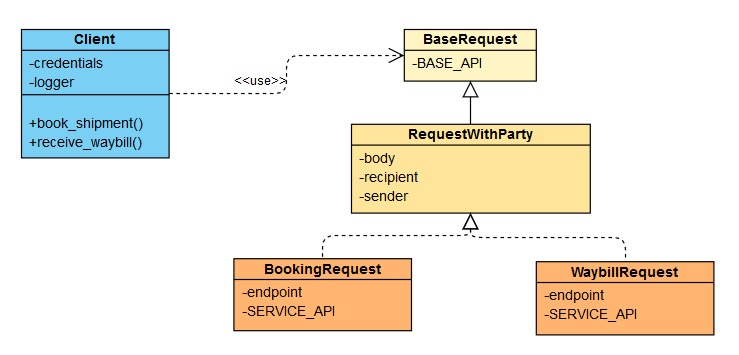
\includegraphics[width=\textwidth]{figures/classdia.png}
    \caption[ClassDia]{Diagramma UML delle classi
    \label{fig:classdia}}
\end{figure}    

Grazie alla gerarchia di classi implementata per le richieste, eventuali modifiche agli \textit{endpoint} sono coperte: ogni membro della gerarchia possiede definisce una parte dell'indirizzo con granularità man mano sempre più fine, partendo dall'URL base del server di SDA nella \texttt{BaseRequest} e arrivando all'URI specifico per la sottoclasse di richiesta desiderata; sono le implementazioni delle richieste finali a comporre l'\textit{endpoint} in fase di inizializzazione, in modo che se viene cambiato ad un passo della gerarchia viene riflesso in tutte le sottoclassi in modo automatico.

\subsubsection{SDA::Client}
I metodi resi disponibili da questa classe eseguono le richieste invocando il metodo privato \texttt{send}, che le invia sfruttando il modulo \ref{itm:http} e controlla la risposta cercando eventuali errori; in caso di esito negativo, ritorna la risposta al metodo che lo ha invocato continuando la normale esecuzione.
\label{tab:sdaattr}
\tabulinesep=5pt
\begin{longtabu} to \textwidth { | c | X | }
        \hline % linea orizzontale
        \hspace{5pt}\textbf{Attributo}\hspace{5pt} & \textbf{Descrizione} \\\hline\hline
        \textbf{\texttt{credentials}} & Credenziali di accesso alle \ref{itm:api} SDA.\cr\hline
        \textbf{\texttt{logger}} & Istanza della classe \texttt{TimestampLogger}.\cr\hline
        \caption{Attributi del \textit{service} \texttt{SDA::Client}.}
\end{longtabu}
\label{tab:sdameth}
\tabulinesep=5pt
\begin{longtabu} to \textwidth { | c | X | }
        \hline % linea orizzontale
        \hspace{5pt}\textbf{Metodo}\hspace{5pt} & \textbf{Descrizione} \\\hline\hline
        \textbf{\texttt{book\_shipment}} & Istanzia ed invia una richiesta \texttt{BookingRequest} di prenotazione di una spedizione, ne elabora la riposta e restituisce il codice di prenotazione.\cr\hline
        \textbf{\texttt{receive\_waybill}} & stanzia ed invia una richiesta \texttt{WaybillRequest} per la lettera di vettura di una spedizione, ne elabora la riposta e restituisce il codice della lettera di vettura e la lettera in formato PDF.\cr\hline
        \caption{Metodi del \textit{service} \texttt{SDA::Client}.}
\end{longtabu}

\subsubsection{SDA::Requests::BaseRequest}
Classe di base, possiede solo l'attributo \texttt{BASE\_API} che fornisce la prima parte dell'indirizzo a cui fare le richieste.

\subsubsection{SDA::Requests::RequestWithParty}
Classe che definisce la base per richieste in cui sono presenti mittente e ricevente; definisce una struttura dati e dei metodi privati per l'estrazione dei dettagli rilevanti dalla farmacia associata alla spedizione e dal file contenente le informazioni di spedizione del laboratorio. Questi metodi vengono invocati in fase di inizializzazione. Inoltre viene dichiarato un metodo virtuale \texttt{generate\_body}, implementato dalle sottoclassi.

\subsubsection{SDA::Requests::BookingRequest}
Classe che definisce la richiesta di prenotazione di una spedizione; l'inizializzazione invoca il costruttore della superclasse, quindi l'implementazione del metodo \texttt{generate\_body} ottenendo il \textit{body} della richiesta a partire dalle strutture dati contenenti mittente e destinatario. Inoltre viene creato l'indirizzo completo dell'\textit{endpoint} concatenando l'attributo ereditato \texttt{BASE\_API} con l'attributo locale \texttt{SERVICE\_API}.

\subsubsection{SDA::Requests::WaybillRequest}
Classe che definisce la richiesta di ottenimento della lettera di vettura per una spedizione; implementata in modo quasi identico a \texttt{BookingRequest}, varia soltanto per la diversa implementazione di \texttt{generate\_body}, che viene adattata al tipo di richiesta.

\subsection{Logger}
Per facilitare le operazioni di debugging dei servizi sopracitati è stato implementato un \textit{logger} in grado di essere istanziato specificando il file in cui salvare il \textit{log} nonché di aggiungere un \textit{timestamp} automaticamente all'evento loggato. Si tratta di un classe molto semplice, che eredita da \texttt{ActiveSupport::Logger} (classe \textit{logger} resa disponibile dal modulo sActive Support) ridefinendone l'attributo \texttt{formatter} (che, appunto, formatta i messaggi registrati nel \textit{log}) aggiungendo il \textit{timestamp}. Il file di \textit{log} viene specificato come parametro del costruttore.

\section{Pannello di amministrazione}
Il pannello di amministrazione è stato progettato ed implementato utilizzando ActiveAdmin, un framework compatibile con Rails che permette di realizzare interfacce amministrative minimizzando il codice necessario.
La progettazione del pannello amministrativo, la cui versione base faceva parte del \textit{back end} preesistente, ha richiesto semplicemente di aggiungere le schede richieste.
\subsection{Struttura delle schede}
Ogni scheda è associata ad un \textit{model}, quindi ad un tipo di record del database; è inoltre possibile ridefinire e restringere lo \textit{scope} dei record visibili da ciascuna scheda.
Esse seguono tutte la stessa struttura:
\begin{itemize}
    \item \textbf{\textit{Model} di riferimento}: viene dichiarato quale \textit{model} viene gestito, con la possibilità di specificarne un alias per chiarezza;
    \item \textbf{Priorità}: ordine di apparizione;
    \item \textbf{Parametri permessi}: vengono dichiarati i parametri modificabili; questo permette di ottenere un controllo a granularità molto fine sulle modifiche al database permesse;
    \item \textbf{\textit{Scope}}: viene dichiarato lo \textit{scope} in forma di \textit{query} sul \textit{model} di riferimento;
    \item \textbf{Filtri}: vengono dichiarati eventuali filtri personalizzati;
    \item \textbf{Azioni}: vengono dichiarate eventuali azioni aggiuntive che sono disponibili per un record, ad esempio il download di un allegato;
    \item \textbf{Indice}: vengono dichiarati gli attributi mostrati nella tabella di indice per ogni record;
    \item \textbf{\textit{Show}}: vengono dichiarati gli attributi mostrati nella visualizzazione di un singolo record;
    \item \textbf{\textit{Form}}: viene dichiarato il form di creazione e modifica dei record, potenzialmente con alcuni campi esclusivi ad una delle due operazioni.
\end{itemize}
\vspace{-15pt}
\subsection{Elenco delle schede}
Di seguito vengono elencate brevemente le schede realizzate o modificate nel corso del progetto:
\tabulinesep=5pt
\begin{longtabu} to \textwidth { | c | X | X |}
        \hline % linea orizzontale
        \hspace{5pt}\textbf{Scheda}\hspace{5pt} & \textbf{\textit{Model}} & \textbf{Azioni speciali}\\\hline\hline
        Admin Users & \texttt{AdminUser} & Nessuna.\cr\hline
        Clienti & \texttt{User} con role ``customer'' & Download dell'eventuale modulo di consenso alla \textit{privacy policy} firmato.\cr\hline
        Gastroenterologi & \texttt{User} con role ``gastroenterologist'' & Reset della password.\cr\hline
        Farmacie & \texttt{Pharmacy} & Nessuna.\cr\hline
        Questionari & \texttt{QuestionnaireTemplate} & Nessuna.\cr\hline
        Sessioni & \texttt{Session} & Nessuna.\cr\hline
        Utenti & \texttt{User} con role ``pharmacist'' & Nessuna.\cr\hline
    \caption{Tabella delle schede del pannello di amministrazione}.
\end{longtabu}


